
\documentclass[10pt]{article} %
\usepackage[preprint]{tmlr}

\title{Re-Thinking Inverse Graphics With Large Language Models}

\author{\name Peter Kulits\textsuperscript{*} \email kulits@tue.mpg.de \\
\addr Max Planck Institute for Intelligent Systems, T{\"u}bingen, Germany
\AND
\name Haiwen Feng\textsuperscript{*} \email hfeng@tue.mpg.de \\
\addr Max Planck Institute for Intelligent Systems, T{\"u}bingen, Germany
\AND
\name Weiyang Liu \email wl396@cam.ac.uk \\
\addr Max Planck Institute for Intelligent Systems, T{\"u}bingen, Germany, University of Cambridge
\AND
\name Victoria Abrevaya \email vabrevaya@tue.mpg.de \\
\addr Max Planck Institute for Intelligent Systems, T{\"u}bingen, Germany
\AND
\name Michael J.~Black \email black@tue.mpg.de \\
\addr Max Planck Institute for Intelligent Systems, T{\"u}bingen, Germany}

\def\month{MM}  %
\def\year{YYYY} %
\def\openreview{\url{https://openreview.net/forum?id=XXXX}} %

\usepackage{graphicx}
\usepackage{color}
\usepackage{symbol}
\usepackage{placeins}
\usepackage{booktabs}
\usepackage{soul}
\usepackage{nicefrac}
\usepackage{wrapfig, tikz}
\usepackage{amsmath,amsfonts,bm,xspace}
\usepackage{bbm}
\usepackage{color}
\usepackage{enumitem, multirow}
\usepackage{fontawesome5}
\usepackage[many]{tcolorbox}
\usepackage{colortbl}


\begin{document}

\blfootnote{\textsuperscript{*}Co-first author}

\maketitle

\begin{abstract}
Inverse graphics -- the task of \textit{inverting} an image into physical variables that, when rendered, enable reproduction of the observed scene -- is a fundamental challenge in computer vision and graphics.
Disentangling an image into its constituent elements, such as the shape, color, and material properties of the objects of the 3D scene that produced it, requires a comprehensive understanding of the environment.
This requirement limits the ability of existing carefully engineered approaches to generalize across domains.
Inspired by the zero-shot ability of large language models (LLMs) to generalize to novel contexts, we investigate the possibility of leveraging the broad world knowledge encoded in such models in solving inverse-graphics problems.
To this end, we propose the Inverse-Graphics Large Language Model (\mbox{\textit{IG-LLM}}), an inverse-graphics framework centered around an LLM, that autoregressively decodes a visual embedding into a structured, compositional 3D-scene representation.
We incorporate a frozen pre-trained visual encoder and a continuous numeric head to enable end-to-end training.
Through our investigation, we demonstrate the potential of LLMs to facilitate inverse graphics through next-token prediction, without the use of image-space supervision.
Our analysis opens up new possibilities for precise spatial reasoning about images that exploit the visual knowledge of LLMs.
We will release our code and data to ensure the reproducibility of our investigation and to facilitate future research at \hbox{\url{https://ig-llm.is.tue.mpg.de/}}
\end{abstract}
\section{Introduction}

\label{sec:intro}

Reconstructing a 3D scene from video is one of the most fundamental problems in vision and has been studied for over five decades.
Today, essentially all state-of-the-art approaches are built on top of Structure-from-Motion (SfM) methods like COLMAP~\cite{schonberger2016structure}. These approaches extract sparse correspondences across frames, match them, discard outliers, and then optimize the correspondences' 3D positions alongside the camera parameters by minimizing reprojection error~\cite{schonberger2016structure}.

This framework has delivered excellent results which underlie many present-day vision applications, and so it is unsurprising that SfM systems have remained largely unchanged in the age of deep learning, save for deep-learning-based correspondence matching \cite{sarlin2020superglue,lindenberger2023lightglue,sarlin2021pixloc,detone2018superpoint}.

However, conventional SfM has a major limitation: it is not differentiable with respect to its free variables (camera poses, camera intrinsics, and per-pixel depths).
This means that SfM acts as an isolated pre-processing step that cannot be embedded into end-to-end deep learning pipelines. 
A differentiable, self-supervised SfM method would enable neural networks to be trained self-supervised on internet-scale data for a broad class of multi-view geometry problems.
This would pave the way for deep-learning based 3D reconstruction and scene understanding.

\begin{figure*}[t]
    \centering
    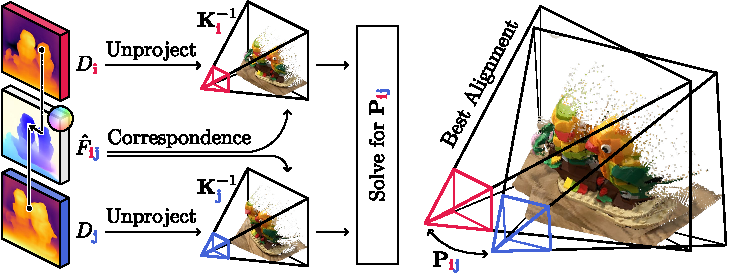
\includegraphics[width=\linewidth,]{figures/procrustes/fig_procrustes_pdf_small.pdf}
    \vspace{-12pt}
    \caption{We solve for the relative poses between consecutive frames using their depth maps, camera intrinsics, and optical flow. To do so, we first unproject their depth maps, then solve for the pose that best aligns the resulting point clouds.}
    \label{fig:procrustes}
    \vspace{-15pt}
\end{figure*}

In this paper, we present FlowMap, a differentiable and surprisingly simple camera and geometry estimation method whose outputs enable photorealistic novel view synthesis. 
FlowMap directly minimizes the difference between optical flow that is induced by a camera moving through a static 3D scene and pre-computed correspondences in the form of off-the-shelf point tracks and optical flow.
Since FlowMap is end-to-end differentiable, it can naturally be embedded in any deep learning pipeline.
Its loss is minimized only via gradient descent, leading to high-quality camera poses, camera intrinsics, and per-pixel depth.
Unlike conventional SfM, which outputs sparse 3D points that are each constrained by several views, FlowMap outputs dense per-frame depth estimates.
This is a critical advantage in downstream novel view synthesis and robotics tasks.
Unlike prior attempts at gradient-based optimization of cameras and 3D geometry~\cite{lin2021barf,nerf--,bian2022nopenerf}, we do not treat depth, intrinsics, and camera poses as free variables.
Rather, we introduce differentiable feed-forward estimates of each one: depth is parameterized via a neural network, pose is parameterized as the solution to a least-squares problem involving depth and flow, and camera intrinsics are parameterized using a differentiable selection based on optical flow consistency.
In other words, FlowMap solves SfM by learning the depth network's parameters; camera poses and intrinsics are computed via analytical feed-forward modules without free parameters of their own.
We show that this uniquely enables high-quality SfM via gradient descent while making FlowMap compatible with standard deep-learning pipelines.
Unlike recent radiance-field bundle-adjustment baselines~\cite{bian2022nopenerf,lin2021barf}, FlowMap does not use differentiable volume rendering, and so it is significantly faster to run, generally reconstructing an object-centric $360^\circ$ scan in less than 10 minutes.

Through extensive ablation studies, we show that each of FlowMap's design choices is necessary.
On popular, real-world novel view synthesis datasets (Tanks \& Temples, Mip-NeRF 360, CO3D, and LLFF), we demonstrate that FlowMap enables photo-realistic novel view synthesis up to full $360^\circ$ trajectories using Gaussian Splatting~\cite{kerbl20233d}. 
Gaussian Splats obtained from FlowMap reconstructions far outperform the state-of-the-art gradient-based bundle-adjustment method, NoPeNeRF~\cite{bian2022nopenerf}, and those obtained using the SLAM algorithm DROID-SLAM~\cite{teed2021droid}, even though both baselines require ground-truth intrinsics.
Gaussian Splats obtained from FlowMap are on par with those obtained from COLMAP~\cite{schonberger2016structure}, even though FlowMap only leverages gradient descent, is fully differentiable, and represents a complete departure from conventional SfM techniques.

\section{Related Work}

\cparagraph{Text-to-Image Generation.}
In recent years, text-to-image generation has made remarkable progress, particularly with the development of diffusion models~\cite{ramesh2022dalle2, nichol2022glide, rombach2022ldm, saharia2022imagen, dhariwal2021diffusionbeatgans, ho2020ddpm, podell2023sdxl, huang2023epidiff} and auto-regressive
models~\cite{chang2023muse, yu2022scalingauto, tian2024var}, which have propelled text-to-image generation to large-scale commercialization. Since DALLE2~\cite{ramesh2022dalle2}, Stable Diffusion~\cite{rombach2022ldm} and Imagen~\cite{saharia2022imagen} employ diffusion models as generative models and train the models on large datasets, text-to-image synthesis ability has been significantly enhanced. More recently, Stable Diffusion XL~\cite{podell2023sdxl}, a two-stage cascade diffusion model, has greatly improved the generation of high-frequency details and overall image color, taking aesthetic appeal to a higher level. However, these existing methods are limited to generating images solely from text prompts, and they do not meet the demand for producing customized images with the preservation of appearance.

\cparagraph{Controllable Image Generation.}
Given the robust generative capabilities of image diffusion models, a series of research~\cite{zhang2023controlnet, mou2023t2iadapter, qin2023unicontrol, ruiz2023dreambooth, hu2021lora, ye2023ipadapter, chen2023anydoor, zhang2024ssrencoder} attempts to explore the controllability of image generation, enabling image synthesis guided by multi-modal conditions. Some work~\cite{zhang2023controlnet, mou2023t2iadapter, jiang2023scedit, qin2023unicontrol, zhao2024unicontrolnet, hu2023cocktail} focuses on introducing structural signals such as edges, depth maps, and segmentation maps, to control the spatial structure of generated images. Another group of work~\cite{ruiz2023dreambooth, hu2021lora, gal2022textualinversion, ye2023ipadapter, chen2023anydoor} uses appearance conditions to guide image generation, aiming to generate images aligning with specific concepts like identity and style, known as subject-driven image generation. The methods generally fall into two categories: those requiring test-time fine-tuning and those that do not. Test-time fine-tuning methods~\cite{ruiz2023dreambooth, hu2021lora, gal2022textualinversion, kumari2023customdiffusion, liu2023cones} often optimizes additional text embedding, parameter residuals or direct fine-tune the whole model to fit the specified subject. Although these methods have achieved impressive results, they cost about half an hour to achieve satisfactory results. Fine-tuning-free methods~\cite{shi2023instantbooth, ye2023ipadapter, chen2023anydoor, zhang2024ssrencoder, ma2023subjectdiffusion, gal2023encoderdiff, wei2023elite} typically train an additional encoding network to encode the reference image into embeddings or image prompts. However, due to the loss of spatial representations when encoding the reference images into one or a few tokens, they struggle to preserve appearance details.

\cparagraph{Controllable Human Image Generation.}
In this paper, we mainly focus on controllable human image generation and aim to synthesize human images aligning with specific text prompts, pose signals, and various parts of human appearance. Text2Human~\cite{jiang2022text2human} generates full-body human images using detailed descriptions about the textures of clothes, but is limited by the coarse-grained textual condition. Test-time fine-tuning methods~\cite{ruiz2023dreambooth,hu2021lora,kumari2023customdiffusion} produce satisfactory results, but when it comes to customizing portraits using multiple parts of human appearance, they take much more time to fit each aspect. Recently, methods like IP-Adapter-FaceID~\cite{ye2023ipadapter}, FastComposer~\cite{xiao2023fastcomposer}, PhotoMaker~\cite{li2023photomaker}, and InstantID~\cite{wang2024instantid} show promising results on zero-shot human image personalization. They encode the reference face to one or several tokens as conditions to generate customized images. With the addition of adaptable structural control networks~\cite{zhang2023controlnet, mou2023t2iadapter}, these methods can generate portraits aligned with specified poses and human identities. However, they usually fail to maintain the details of human identities and utilize all the information from a single image, resulting in ambiguous subject representation. These make it difficult to apply these schemes to precisely generation conditioned on multiple parts of the human appearance. In contrast, our Parts2Whole is both generalizable and efficient, and precisely retains details in multiple parts of human appearance.
\section{Method}

In this section, we detail our STAR-MT method and the domain adaptation benchmark. The overall scheme of the proposed solution is illustrated in Fig.\ref{fig:SFVOD}. 

\subsection{Mean-teacher for domain adaptive VOD}
 In developing our method, we leverage the advanced unsupervised domain adaptation strategies found in the mean-teacher self-training approach \cite{tarvainen2017mean}. We introduce the implementation of this method in this paradigm.
 
 As a class of student-teacher training approach, the mean-teacher method keeps two identical networks: the student network and the teacher network. They are initialized by the weights trained on the source domain. During training, the weights of the teacher model are fixed, while the student model is trained with the supervision signal from the prediction output and features generated from the teacher model. On the other hand, the teacher model takes the exponential moving average (EMA) of consecutive student models for its parameter update:
\begin{equation}
    \theta_{\mathcal{T}}^{t} \leftarrow \alpha \theta_{\mathcal{T}}^{t-1} + (1-\alpha) \theta_{\mathcal{S}}^{t-1},
\end{equation}
where the $\theta_{\mathcal{T}}$ and $\theta_{\mathcal{S}}$ denote the weights of teacher and student models, $t$ denotes the training iteration, and $\alpha \in (0,1)$ is the momentum coefficient which is usually set close to 1 for a smooth temporal ensemble \cite{cao2023contrastive}.
 
\subsection{Spatial-Temporal Alternate Refinement}
YOLOV utilized the pre-trained backbone of YOLOX as its frame-wise feature extractor, followed by feature selection and affinity measurement that identifies features from the same object among frames to guide temporal aggregation. However, training the spatial backbone and temporal aggregation module simultaneously on the video object detection dataset is suboptimal because they require different training schemes. Hence, we propose to adapt the YOLOV in a two-stage alternate optimization manner, consisting of the temporal refinement stage (TRS) and spatial refinement stage (SRS).

\subsubsection{Temporal Refinement Stage (TRS).}
In the TRS, the entire teacher model, including the frame-wise backbone and temporal aggregation module, is updated via EMA. In the beginning, both teacher and student models are initialized the same.
Like a typical mean-teacher-based algorithm, the same image sequences with different augmentations are fed into those models. The teacher model processes the weakly augmented images, and the heavily augmented images are fed into the student model. Moreover, we randomly mask out $r\%$ frames and enforce the student model to produce the same output with fewer frames than the teacher model. This masking mechanism can supposedly enhance the generalization capability of temporal aggregation. The student model is trained by aligning frame-wise features and soft pseudo labels with the features and predictions of the teacher model. The loss in this stage is defined as:
\begin{equation}
    \mathcal{L} = \mathcal{L}_{MSE}(f_{\mathcal{T}}, f_{\mathcal{S}}) + \mathcal{L}_{BCE}(y_{\mathcal{T}}^{cls}, y_{\mathcal{S}}^{cls}),
\end{equation}
where the first term is the mean square error between the feature maps $f_{\mathcal{T}}$ and $f_{\mathcal{S}}$, produced by the backbone module of the teacher and student models, respectively. The term $\mathcal{L}_{BCE}$ denotes the binary cross entropy loss. $y_{\mathcal{T}}^{cls}$ refers to the top-$k$ classification prediction after the temporal aggregation of the teacher model, and $y_{\mathcal{S}}^{cls}$ refers to that of the student model. $k$ is the number of proposals in the feature selection module before the temporal aggregation. We set $k=30$ following the default setting of YOLOV. We do not particularly compute the loss of objectiveness and bounding box prediction because they are unchanged in the temporal aggregation module. 


\subsubsection{Spatial Refinement Stage (SRS).} 
TAM consists of two key components: a Feature Selection Module, which selects high-quality prediction proposals, and a Feature Aggregation Module, which fuses these proposals across multiple frames. However, due to the inconsistency between the training pipelines of the single-frame detection head (backbone) and the TAM, the TRS, which mostly follows the training setting of the TAM, may lead to suboptimal adaptation on the backbone side. Recognizing that the TAM can reliably improve prediction quality, we propose using the output class score of YOLOV, instead of YOLOX, in the teacher model as higher-quality pseudo labels to guide the fine-tuning of the detection head of YOLOX in the student model. In the SRS, only the backbone of the teacher model is updated via EMA, ensuring that the adaptation focuses on the spatial feature extraction process while leveraging the enhanced temporal information from the TAM. The loss is given as follows:
\begin{equation}
    \mathcal{L} = \mathcal{L}_{MSE}(f_{\mathcal{T}}, f_{\mathcal{S}}) + \mathcal{L}_{BCE}(y_{\mathcal{T}}^{cls}, y_{\mathcal{S}}^{cls}) + \gamma \mathcal{L}_{cls},
\end{equation}

\noindent where $\gamma$ is the weighting factor. The new loss term $\mathcal{L}_{cls}$ is the certainty-aware binary cross entropy loss between the filtered class score from the teacher and student model:
\begin{equation}
\begin{aligned}
    \mathcal{L}_{cls}  = -\frac{1}{N}\sum_{i}^{N} p^{i}_{\mathcal{S}} \Big[ \frac{1}{n_{c}} & \sum_{c}^{n_c}  \left( s_{\mathcal{T}}^{i,c} \log(s_{\mathcal{S}}^{i,c}) \right. \\
    & \left.  +(1-s_{\mathcal{T}}^{i,c}) \log(1-s_{\mathcal{S}}^{i,c}) \right) \Big],
\end{aligned}
\end{equation}
\noindent where $c$ is the index of the category, $n_c=30$ is the number of classes, and $i$ and $N$ are the index and number of detected objects in the sequence. $s_{\mathcal{S}}^{i,c}$ and $s_{\mathcal{T}}^{i,c}$ are the $i$-th output scores of class $c$ for the student and teacher models, respectively. $p^{i}_{\mathcal{S}} \in (0,1)$ is the normalized objectiveness score in the student model output, serving as the weight of the pseudo-label. It can be viewed as the certainty measurement of the object's existence; the greater $p^{i}_{\mathcal{S}}$ indicates the higher confidence of the particular pseudo label.
 
\subsubsection{Alternate Refinement.} 
STAR-MT training is periodical, with the TRS and SRS having identical iterations $\tau$ in each period. Given $k$ the index of the period, TRS is executed in iterations $[2k\tau, 2k\tau+\tau)$ and SRS in iterations $[2k\tau+\tau, 2k\tau+2\tau)$. During the experiment, it was observed that the order of those two stages only had a trivial impact on the overall performance.

Although early stopping is not explicitly implemented in our approach, we utilize the mean self-entropy \cite{li2021free} of the class score from the teacher model as a performance criterion for all output checkpoints. This mean self-entropy, denoted as $H$, serves as a measure of reliability for pseudo labels; a lower $H$ indicates greater confidence in the teacher model in guiding the student. The checkpoint corresponding to the minimal value of $H$ is selected as our output model. The formula to compute $H$ is as follows:
\begin{equation}
    H  = -\frac{1}{Nn_{c}} \sum_{i}^{N}  \sum_{c}^{n_c} s_{\mathcal{T}}^{i,c} \log(s_{\mathcal{T}}^{i,c}).
\end{equation}
\section{Evaluations}\label{sec:evaluations}
\begin{figure}[t]
\centering
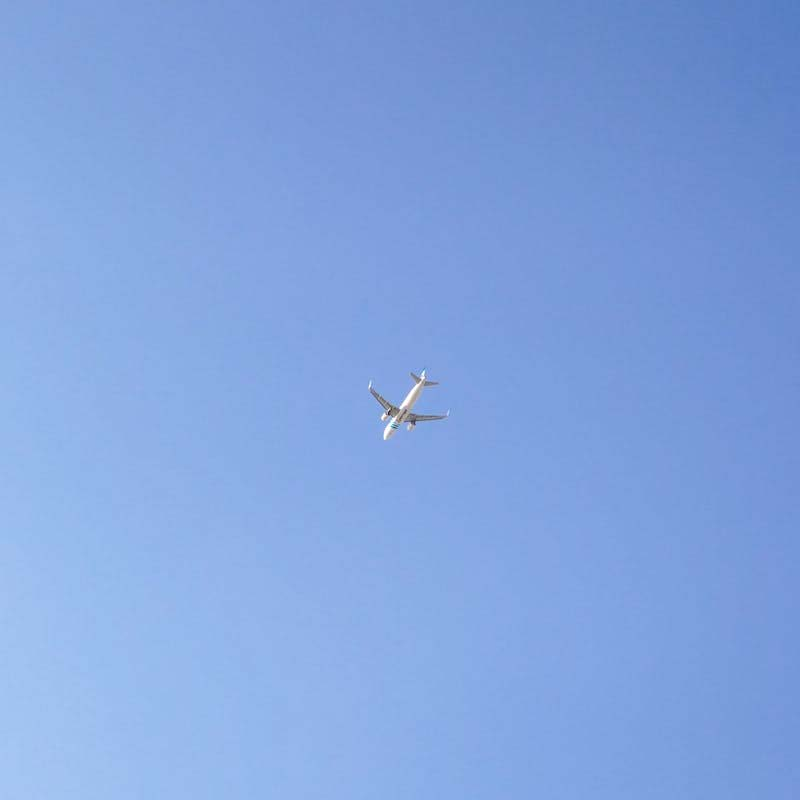
\includegraphics[width=0.2475\linewidth]{figures/airplane/6dof/input/0.jpg}\hfill
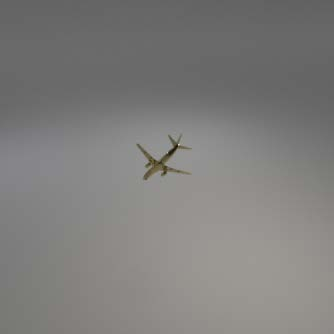
\includegraphics[width=0.2475\linewidth]{figures/airplane/6dof/output/0.jpg}\hfill
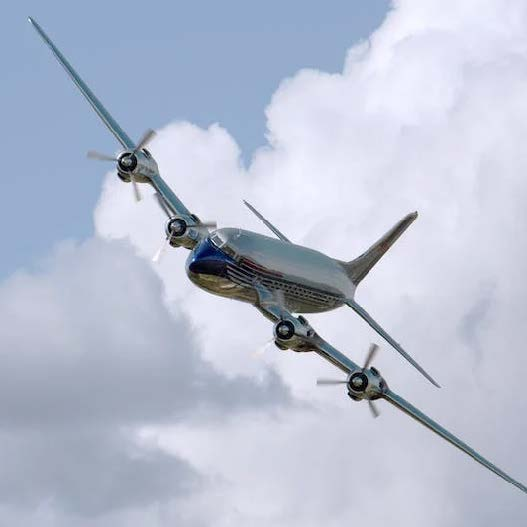
\includegraphics[width=0.2475\linewidth]{figures/airplane/6dof/input/1.jpg}\hfill
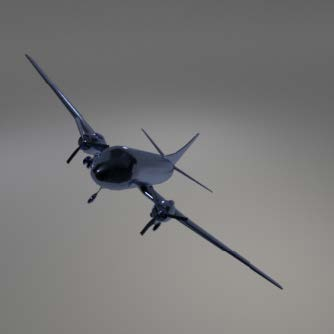
\includegraphics[width=0.2475\linewidth]{figures/airplane/6dof/output/1.jpg}
\caption{\textbf{OOD Single-Object 6-DoF Samples.} (\cref{sssec:single_6dof})
A sample 6-DoF reconstruction of real-world images.
The model is finetuned with only Blender renderings of toy airplanes that have a white backdrop.
See \cref{fig:single_6dof_samples_additional} for additional samples.
}
\label{fig:single_6dof_samples}
\end{figure}
To evaluate the ability of our proposed framework to generalize across distribution shifts, we design a number of focused evaluation settings.
We conduct experiments on synthetic data in order to quantitatively analyze model capability under controlled shifts.

\subsection{Compositional Generalization on CLEVR}\label{ssec:clevr}
An extension to CLEVR, known as CLEVR-CoGenT~\citep{johnson2017clevr}, serves as a benchmark for evaluating the \textit{compositional}-generalization capabilities of VQA models.
This benchmark assesses the model's ability to answer questions about scenes containing objects with unseen combinations of attributes.
During training, the dataset is structured such that particular types of objects are only assigned specific combinations of attributes (e.g.~blue cubes and red cylinders), while the testing data includes objects with attribute combinations not seen during training (e.g.~red cubes and blue cylinders).
We adapt this VQA dataset to our inverse-graphics problem domain, employing it for three primary purposes:
1) demonstrating that LLMs can effectively perform inverse graphics by testing on in-distribution (ID) data;
2) illustrating that LLMs exhibit robust compositional generalization to OOD data, while the baseline approach in NS-VQA~\citep{yi2018neural} struggles in this setting; and
3) exploring the data-efficiency of our framework.

\noindent\textbf{Setting.}
Following the setting of CLEVR-CoGenT, our training set consists of images of scenes containing objects with only a subset of possible attribute combinations (shape, size, material, and color).
In the ID condition, all cubes are rendered in gray, blue, brown, or yellow, and all cylinders are depicted in red, green, purple, or cyan.
In contrast, in the OOD condition the color palettes of the shapes are swapped.
Spheres are consistently depicted with all eight colors under both conditions.
We train both our proposed framework and NS-VQA, our neural-scene de-rendering baseline, on 4k images from the ID condition and evaluate them on 1k images from both the ID and OOD conditions. We follow CLEVR and randomly apply their set of synonyms on the categorical attributes.

\begin{table}[t]
\centering
\caption{
\textbf{CLEVR-CoGenT Results.} (\cref{ssec:clevr})
While both our proposed framework and the baseline, NS-VQA, and are able to achieve \textgreater 99\% accuracy on the ID condition, the baseline fails to generalize, with its shape-recognition accuracy dropping by 66.12\%.
\textit{Color}, \textit{Mat.}, and \textit{Shape} represent respective accuracies and $\uparrow$ indicates greater is better.
}
\begin{tabular}{lrrr|rrr}
\toprule
& \multicolumn{3}{c}{ID} & \multicolumn{3}{c}{OOD} \\
& Char & Float & NS-VQA & Char & Float & NS-VQA \\
\midrule
$\downarrow$L2 & 0.21 & 0.16 & 0.18 & 0.22 & 0.17 & 0.18 \\
$\uparrow$Size & 99.71 & 99.77 & 100.00 & 99.74 & 99.80 & 100.00 \\
$\uparrow$Color & 99.58 & 99.71 & 100.00 & 98.60 & 98.14 & 99.95 \\
$\uparrow$Shape & 99.51 & 99.59 & 100.00 & 93.50 & 93.14 & \fbox{33.88} \\
\bottomrule
\end{tabular}
\label{table:clevr}
\end{table}

\noindent\textbf{Evaluation Metrics.}
To evaluate attribute-recognition accuracy, we employ linear-sum assignment on pairwise Euclidean distances to match predicted and ground-truth objects.
However, since attribute-recognition accuracy does not account for missing or duplicated objects, we also evaluate the method's ability to produce accurate counts by computing the mean-absolute counting error between the predicted and ground-truth object sets across scenes (\textit{Count}).

\begin{wrapfigure}{R}{0.45\linewidth}
\centering
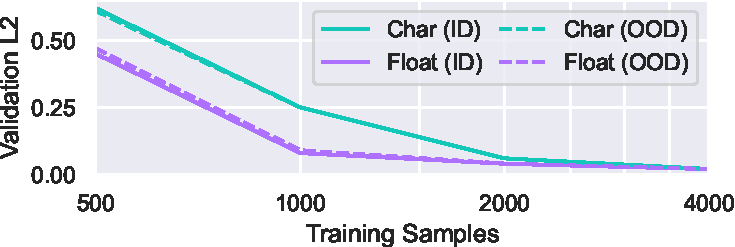
\includegraphics[width=\linewidth]{figures/clevr/data_efficiency_plot.pdf}
\caption{\textbf{CLEVR Data Efficiency.} (\cref{ssec:clevr})
Plot of the validation L2 positional error by the number of training samples.
We observe that the float-based model is consistently more data-efficient but that the difference between the models converges as the number of training samples reaches 4000.
See \cref{table:clevr_data_efficiency} for a full quantitative comparison.
}
\label{fig:clevr_data_efficiency}
\vspace{-0.5cm}
\end{wrapfigure}
\noindent\textbf{Results.}
Both our proposed framework and NS-VQA achieve \textgreater 99\% accuracy on the ID condition (\cref{table:clevr}), which underscores LLMs' ability to perform comparably with domain-specific modular designs.
However, when evaluated on the OOD condition, the shape-recognition accuracy of the baseline method drops substantially by 66.12\%, while the accuracy of our pipeline decreases by only 6.01\%.
Notably, when spheres, observed with all colors during training, are removed from the evaluation, the shape accuracy of NS-VQA plummets further to 0.03\%.
Illustrative reconstructions from the OOD condition can be seen in \cref{fig:clevr_samples}.

In terms of data efficiency, we find the float-based model to be much more efficient than the char-based model in estimating the positions of objects, but the difference diminishes as the number of samples reaches 4k (\cref{fig:clevr_data_efficiency}).
Hypothesizing that the char-based model has learned to compositionally retrieve the exact positions of (individual) objects from the training set rather than learning to effectively interpolate between training values, we measure 
the likelihood of predicting arbitrary three-decimal values.
Our findings reveal that the char-based model is 6.41 times more likely to predict a particular value if that discrete value was observed during training.
We further explore float-estimation dynamics in \cref{ssec:parameter_space_generalization}.

\subsection{Numeric Parameter-Space Generalization}\label{ssec:parameter_space_generalization}
In this section, we investigate the addition of a numeric head and the ability of our framework to generalize across parameter space.

\begin{figure*}[t]
\centering
\begin{subfigure}{.196\linewidth}
\centering
\raisebox{0cm}{
\includegraphics[width=\linewidth]{figures/2d/sparse_checkerboard.pdf}}
\caption{Train Distribution}\label{fig:2d_sparse_checkerboard}
\end{subfigure}
\hspace{-0.15cm}
\begin{subfigure}{.196\linewidth}
\centering
\raisebox{0cm}{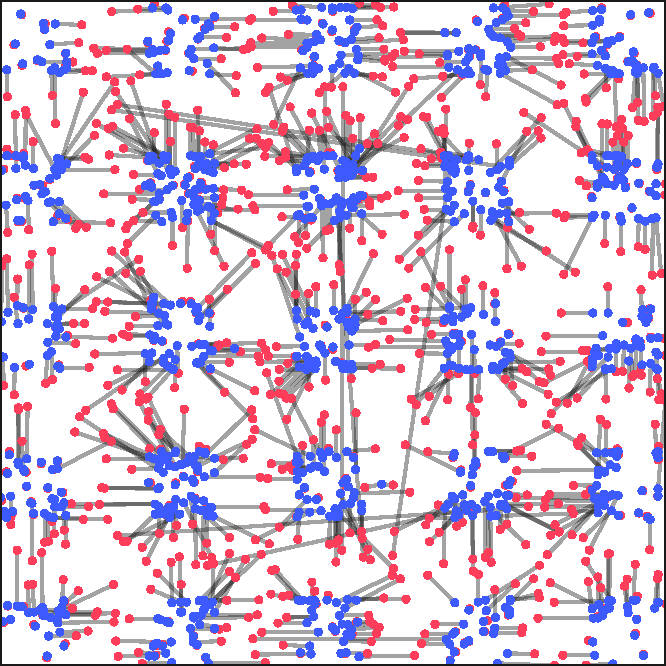
\includegraphics[width=\linewidth]{figures/2d/char_scatter.pdf}}
\caption{Char Model Pred.}\label{fig:2d_char_scatter}
\end{subfigure}
\hspace{-0.15cm}
\begin{subfigure}{.196\linewidth}
\centering
\raisebox{0cm}{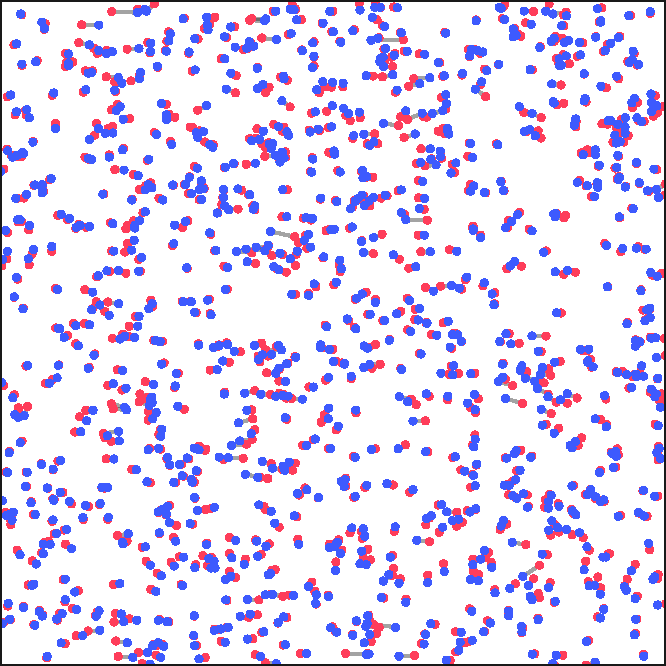
\includegraphics[width=\linewidth]{figures/2d/float_scatter.pdf}}
\caption{Float Model Pred.}\label{fig:2d_float_scatter}
\end{subfigure}
\begin{subfigure}{.196\linewidth}
\centering
\raisebox{0.0cm}{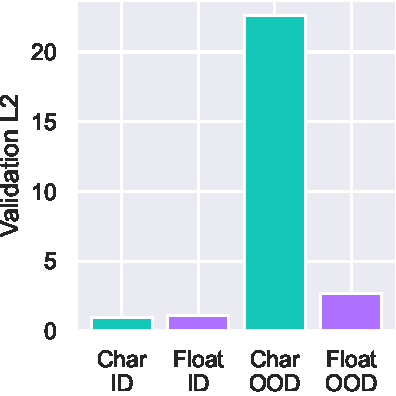
\includegraphics[width=\linewidth]{figures/2d/bar.pdf}}
\caption{ID--OOD}
\label{fig:2d_bar}
\end{subfigure}
\hfill
\begin{subfigure}{.196\linewidth}
\centering
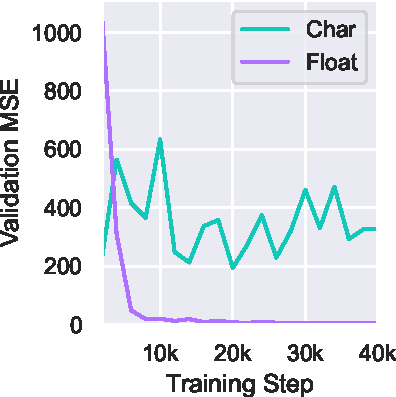
\includegraphics[width=\linewidth]{figures/2d/dynamics.pdf}
\caption{Dynamics}
\label{fig:2d_dynamics}
\end{subfigure}
\caption{\textbf{2D Parameter-Space Generalization.} (\cref{sssection:2d})
(a) Training positions are sampled from the checkerboard.
When evaluated on images with uniformly sampled positions, the char-based model fails to generalize outside the training distribution (b) while the float-based model effectively interpolates samples (c).
Randomly-sampled testing locations are shown in red and the corresponding predictions in blue.
(d) shows that while both methods well-estimate samples from the ID condition, the char-based model struggles to generalize.
(e) shows a plot of the model's validation MSE as a function of the number of training steps.
We observe that the training of the float-based model is much smoother and converges quickly.
}
\label{fig:2d}
\end{figure*}

\subsubsection{2D Parameter Space}\label{sssection:2d}
We begin by scrutinizing the framework's ability to generalize in 2D parameter space across range gaps.
To accomplish this, we create a dataset comprising 10k images, each featuring a red dot on a white background.
During training, the model is shown images where the location of the dot is sampled from a sparse checkerboard grid, as shown in \cref{fig:2d_sparse_checkerboard}.
During evaluation, the model is shown 1k images where the dot's location is uniformly sampled across the square; points lying outside the checkerboard are effectively OOD inputs. 

\noindent\textbf{Results.}
As shown in \cref{fig:2d_char_scatter}, the char-based model exhibits significant overfitting to the training distribution, consistently predicting dot locations restricted to the checkerboard distribution observed during training.
In contrast, the float-based model is able to effectively generalize across parameter space, adapting to the uniformly sampled testing distribution during evaluation (\cref{fig:2d_float_scatter}).
Although the float-based model exhibits a slight positional bias toward predicting positions on the grid (as evidenced by the higher OOD error),  
the disparity in the ID--OOD validation-L2 performance gap of the char-based model is 14 times as high as that of the float-based model (\cref{fig:2d_bar}).
Moreover, the validation MSE of the float-based model converges quickly to near zero, while the error of the char-based model is much less stable over time (\cref{fig:2d_dynamics}), suggesting that the float-based model learns smooth, low-dimensional representations of the space while the char-based variant may not.

\subsubsection{SO(3) Parameter Space}\label{sssec:so3}
\begin{figure}
\centering
\fbox{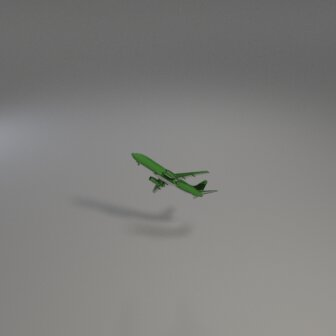
\includegraphics[width=0.4\linewidth]{figures/samples/so3.jpg}}
\begin{minted}[breaklines]{python}
add(shape='airliner', size='tiny', color='green', material='matte', rotation=(-0.798, 0.124, 0.590, -0.562, -0.507, -0.654))
\end{minted}
\caption{\textbf{SO(3) Range-Gap Train Sample.} (\cref{sssec:so3})}
\label{fig:code_so3}
\end{figure}
We continue our parameter-space evaluation within the more complex task of SO(3)-pose estimation of orientable objects.
For this, we make use of five toy-airplane assets sourced from Super-CLEVR~\citep{Li_2023_CVPR}. 
We construct a training dataset of 10k images of single planes at a fixed location and sampled attributes identical to those in CLEVR.
Extending the range-gap setup used in \cref{sssection:2d}, the airplanes are assigned random extrinsic-Euler rotations, where the components are sampled from ranges containing inserted gaps (e.g., $[-\frac{\pi}{20},\frac{\pi}{20}]$).
A visual depiction of this space is provided in \cref{fig:so3_range}, with the training values exclusively sampled from the blue ranges.
During testing, we invert the gaps to assess OOD generalization.
We evaluate performance across intrinsic-Euler, extrinsic-Euler, axis-angle, and 6D~\citep{Zhou_2019_CVPR} representations.

\noindent\textbf{Results.}
We report full results in \cref{table:so3} and here discuss only results from the best-performing representation variants in each evaluation, being intrinsic-Euler for char and 6D for float in ID, and axis-angle for both in OOD.
We do so to avoid biasing results with a representation that is better suited for one model variant or the other.

As depicted in \cref{fig:so3_bar}, the error of the char-based model is 2.64 times higher than that of the float-based model when evaluated in-distribution.
Upon testing in the OOD condition, the disparity is nearly consistent at 2.52 times that observed in the ID scenario, with the ID--OOD gap of the char-based model being 2.21 times that observed in the float-based variant.
We attribute the superiority of the float-based model across both conditions to the increased data dimensionality.
Additionally, the lesser performance decline observed when evaluating on the OOD training gaps further underscores the parameter-space efficiency of the float-based model.

\subsection{6-DoF Pose Estimation}\label{ssec:6dof}
\begin{figure}[t]
\centering
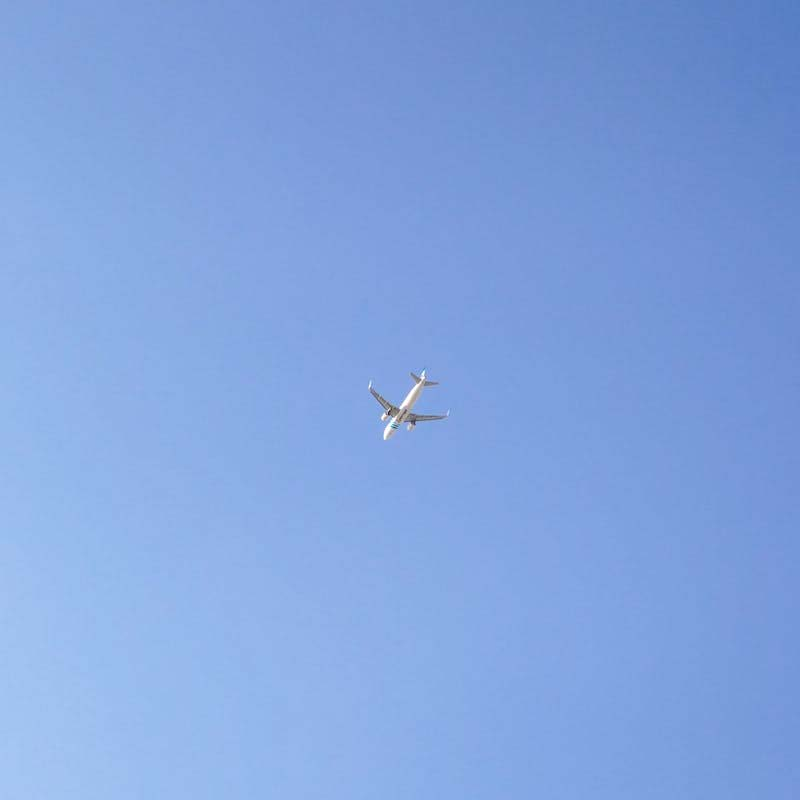
\includegraphics[width=0.2475\linewidth]{figures/airplane/6dof/input/0.jpg}\hfill
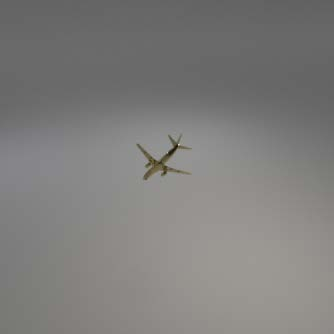
\includegraphics[width=0.2475\linewidth]{figures/airplane/6dof/output/0.jpg}\hfill
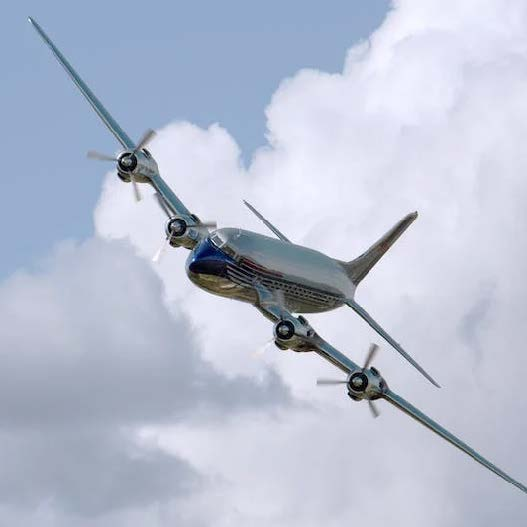
\includegraphics[width=0.2475\linewidth]{figures/airplane/6dof/input/1.jpg}\hfill
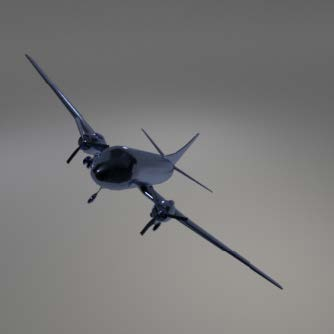
\includegraphics[width=0.2475\linewidth]{figures/airplane/6dof/output/1.jpg}
\caption{\textbf{OOD Single-Object 6-DoF Samples.} (\cref{sssec:single_6dof})
A sample 6-DoF reconstruction of real-world images.
The model is finetuned with only Blender renderings of toy airplanes that have a white backdrop.
See \cref{fig:single_6dof_samples_additional} for additional samples.
}
\label{fig:single_6dof_samples}
\end{figure}
We examine the ability of our framework to scale in tackling a more challenging inverse-graphics task: that of 6-DoF-pose estimation.
Our exploration begins with an evaluation on single-object images, encompassing both quantitative and qualitative assessments, where we illustrate the framework's ability to generalize across visual domain shifts.
We subsequently extend the setting to include more-complex (albeit, synthetic) multi-object scenes, demonstrating promising results for scene estimation, handling larger collections (\textgreater 100) of diverse assets. 
\begin{table}[t]
\centering
\caption{
\textbf{CLEVR-CoGenT Results.} (\cref{ssec:clevr})
While both our proposed framework and the baseline, NS-VQA, and are able to achieve \textgreater 99\% accuracy on the ID condition, the baseline fails to generalize, with its shape-recognition accuracy dropping by 66.12\%.
\textit{Color}, \textit{Mat.}, and \textit{Shape} represent respective accuracies and $\uparrow$ indicates greater is better.
}
\begin{tabular}{lrrr|rrr}
\toprule
& \multicolumn{3}{c}{ID} & \multicolumn{3}{c}{OOD} \\
& Char & Float & NS-VQA & Char & Float & NS-VQA \\
\midrule
$\downarrow$L2 & 0.21 & 0.16 & 0.18 & 0.22 & 0.17 & 0.18 \\
$\uparrow$Size & 99.71 & 99.77 & 100.00 & 99.74 & 99.80 & 100.00 \\
$\uparrow$Color & 99.58 & 99.71 & 100.00 & 98.60 & 98.14 & 99.95 \\
$\uparrow$Shape & 99.51 & 99.59 & 100.00 & 93.50 & 93.14 & \fbox{33.88} \\
\bottomrule
\end{tabular}
\label{table:clevr}
\end{table}
\subsubsection{Single-Object 6-DoF}\label{sssec:single_6dof}
We first evaluate our framework's ability to scale to single-object 6-DoF pose estimation. The float- and char-based models are assessed quantitatively using rendered images. 

\noindent\textbf{Setting.}
We extend the setting used in \cref{sssec:so3} but unfreeze the previously fixed 3D position and assign it a randomly sampled value.
We expand the number of colors used in the dataset to 133\footnote{\url{https://simple.wikipedia.org/wiki/List_of_Crayola_crayon_colors}} to better emulate the diversity observed in the real world.
Differing from the previous setup, we fix the size of the objects due to the relative depth--scale ambiguity of the toy airplanes.
To evaluate our framework's ability to scale beyond data-constrained scenarios, we render a training dataset of one-million images.
Following the rotation-representation results of \cref{sssec:so3}, we use the intrinsic-Euler representation for the char-based model and the 6D representation for the float-based model as their use led to the greatest ID performance.

\noindent\textbf{Results.}
\cref{table:single_6dof} illustrates that, under this non-data-constrained scenario, both model variants effectively capture the dynamics of the task
The models both notably exhibit an order of magnitude lower positional error than in the CLEVR setting, despite the addition of 3D orientation and an additional positional dimension, and achieve rotational error 28\% of that observed in the ID portion of the SO(3) range-gap evaluation.
This reinforces the earlier observation from the CLEVR data-efficiency evaluation that, given sufficient data, the model variants exhibit a similar performance ceiling.
Still, neither achieves the level of precision necessary to be directly constrained by the three-decimal-place discretization applied to numeric quantities throughout the evaluations nor the 16-bit training precision in the case of the float-based model.
See \cref{sec:further_training_details} for further training details.

As part of our evaluation, we also qualitatively examine the ability of the model to transfer from the renders of toy planes with a solid-white background, on which it was fine-tuned, to estimating the pose and attributes of planes in real-world images.
We provide qualitative samples of our model's generalization to such images in \cref{fig:single_6dof_samples}.
We observe encouraging generalization across the majority of images tested, despite the lack of augmentation or domain-specific inductive bias applied during the training process.
However, it is difficult to quantitatively evaluate such model performance due to a lack of paired real-world data in line with our compositional task.
As a proxy for such an evaluation, we introduce a synthetic setting in \cref{sssec:scene_6dof} to quantitatively evaluate the ability of our framework to generalize across visual domains.

\subsubsection{Scene-Level 6-DoF}\label{sssec:scene_6dof}
\begin{table}[t]
\centering
\caption{
\textbf{CLEVR-CoGenT Results.} (\cref{ssec:clevr})
While both our proposed framework and the baseline, NS-VQA, and are able to achieve \textgreater 99\% accuracy on the ID condition, the baseline fails to generalize, with its shape-recognition accuracy dropping by 66.12\%.
\textit{Color}, \textit{Mat.}, and \textit{Shape} represent respective accuracies and $\uparrow$ indicates greater is better.
}
\begin{tabular}{lrrr|rrr}
\toprule
& \multicolumn{3}{c}{ID} & \multicolumn{3}{c}{OOD} \\
& Char & Float & NS-VQA & Char & Float & NS-VQA \\
\midrule
$\downarrow$L2 & 0.21 & 0.16 & 0.18 & 0.22 & 0.17 & 0.18 \\
$\uparrow$Size & 99.71 & 99.77 & 100.00 & 99.74 & 99.80 & 100.00 \\
$\uparrow$Color & 99.58 & 99.71 & 100.00 & 98.60 & 98.14 & 99.95 \\
$\uparrow$Shape & 99.51 & 99.59 & 100.00 & 93.50 & 93.14 & \fbox{33.88} \\
\bottomrule
\end{tabular}
\label{table:clevr}
\end{table}
\begin{figure}[t]
\centering
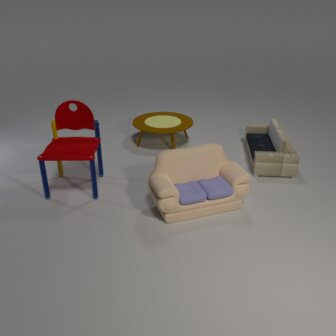
\includegraphics[width=0.2475\linewidth]{figures/shapenet/OOD/0_in.jpg}\hfill
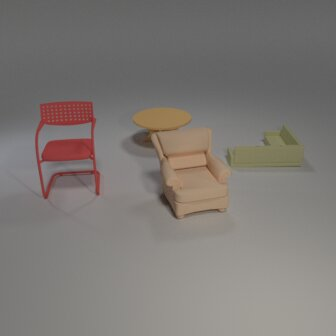
\includegraphics[width=0.2475\linewidth]{figures/shapenet/OOD/0_out.jpg}\hfill
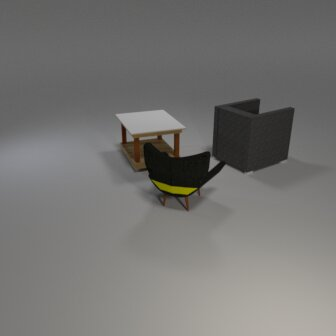
\includegraphics[width=0.2475\linewidth]{figures/shapenet/OOD/1_in.jpg}\hfill
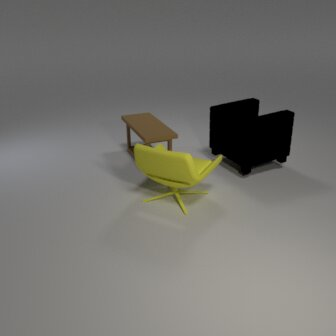
\includegraphics[width=0.2475\linewidth]{figures/shapenet/OOD/1_out.jpg}
\caption{\textbf{OOD ShapeNet 6-DoF Samples.} (\cref{sssec:scene_6dof})
Two sample reconstructions from the OOD ShapeNet 6-Dof pose-estimation experiment.
Left to right: input, output.
We evaluate on assets not shown during training, with out-of-distribution textures.
See \Cref{fig:scene_6dof_ood_samples_additional} for additional samples.
}
\label{fig:scene_6dof_ood_samples}
\end{figure}
In this section, we explore the scalability of our framework to scene-level 6-DoF-pose estimation, featuring 3-5 objects per scene and a much-expanded array of assets.
This experiment not only assesses performance under more-challenging conditions, but also enables a quantitative evaluation on the framework's ability to generalize to scenes with OOD visual appearance.

\noindent\textbf{Setting.}
We construct an expanded CLEVR-like image--scene dataset, incorporating objects sourced from ShapeNet~\citep{shapenet2015}.
The dataset comprises 56 chair types, 35 sofa types, and 47 table types.
We remove the size and material attributes used in CLEVR, but employ the expanded color set used in \cref{sssec:single_6dof} to randomly color the objects.
After doing so, the total number of possible combinations of attributes is 191-fold that used in the CLEVR-CoGenT experiment.
Differing from previous evaluations, we also vary the pitch of the camera and the radius of its arc, but maintain a fixed camera focal point.
Returning from the million-image single-object 6-DoF evaluation to a relatively data-constrained setting, we render 10k training images and evaluate the framework on three conditions, each with 1K images:
(1) ID, which matches the training distribution of scenes with solid-colored objects;
(2) OOD texture (OOD-T), where the same object assets are used as in ID but the objects are rendered with original ShapeNet textures instead of the randomly assigned solid colors;
and (3) OOD encompassing both unseen objects and original ShapeNet textures (OOD-T+S). We use this to emulate the distribution shift of modeling real-world scenes, while facilitating quantitative evaluation.

\noindent\textbf{Results.}
We observe that both approaches scale to the task, though the float-based model outperforms -- or ties with -- the char-based variant across evaluations (\cref{table:scene_6dof}).
This disparity is emphasized in the OOD-T+S setting where scene-level chamfer distance of the char-based model jumps from being approximately twice that of the float-based variant in the ID and OOD-T evaluations to being 5.67 times as much.

There is a decrease in performance observed when stepping to the OOD-T setting, which is most-strongly observed in the count error (x8 for both) and the shape-recognition accuracy (-20.49\% in char and -15.05\% in float).
We empirically attribute this to the model occasionally explaining some multi-color textured objects using a composition of multiple, solid-color assets.
Quantitatively supporting this, the performance decrease is not as strongly reflected in scene-level chamfer distance (x2.6 for both).

See \cref{fig:scene_6dof_ood_samples} for samples reconstructions from OOD-T+S and \cref{fig:scene_6dof_id_samples_additional} for samples from the ID setting.
We additionally test our model on real-world samples, but find that it fails to consistently generalize (\cref{fig:scene_6dof_rw_samples}).
We attribute this failure partially to limitations in the camera-position training distribution.
\section{Discussion and Limitations}
Through our investigation, we demonstrated the ability of LLMs to facilitate inverse-graphics tasks across a variety of domain shifts, albeit within controlled settings.
In designing targeted evaluations to analyze the model's generalization ability, our goal was to lay the groundwork necessary for future advancements.
However, scaling up these models to metrically reconstruct complex real-world scenes will undoubtedly pose additional challenges.

The primary limitation of our approach lies in that its expressiveness is constrained by the expressiveness of the training-data-generation framework.
We demonstrated its ability to learn to compositionally disentangle images of scenes into constituent elements, reconstructing scenes under distribution shifts.
However, reproducing scenes as text, it can reconstruct scenes containing unknown objects in OOD configurations, but it does so in terms of the objects -- and language -- it is trained with.
If it does not know the name of asset \mbox{\texttt{chairs\_0055}}, it will not be able to use it.
Even if the model produces the name of a new color or shape from outside of the training data, the graphics engine rendering the LLM output must have an understanding of it in order to apply it.

In contrast, the generality of our approach, which doesn't incorporate special task-specific inductive biases, allows it to scale with the diversity of the training data or the expressivity of the code format.
Future work may explore more-scalable training-data generators or integrate self-supervision techniques to enable learning from unlabeled images.
While we employ a relatively straightforward object-centric code representation across experiments for simplicity, more-expressive scene representations should also be explored.

Our evaluation scenes feature only minor object occlusions and are relatively simple.
While a generic next-token objective paired with MSE float supervision sufficed for these scenarios, addressing harder-to-disentangle scenes may require a trade-off between generality and inductive bias, to incorporate additional supervision.
\section{Conclusion}
In this work, we investigated the ability of LLMs to solve inverse-graphics challenges.
Introducing the Inverse-Graphics Large-Language-Model (IG-LLM) framework, we demonstrated that the broad generalization and reasoning capabilities of LLMs can be harnessed to facilitate inverse-graphics tasks.
Through extensive evaluation, we assessed the model's capacity to generalize out-of-domain, revealing its ability to abstract scene elements compositionally.
We additionally explored the integration of a numeric head to adapt LLMs for continuous metric-value estimation, providing enhanced generalization and smoother training dynamics.
Our quantitative analyses demonstrate its ability to generalize compositionally (\cref{ssec:clevr}), in parameter space (\cref{ssec:parameter_space_generalization}), and across visual domains (\cref{ssec:6dof}).
Our investigation demonstrates the ability of IG-LLM to leverage the general knowledge of LLMs in solving inverse-graphics problems, opening a new avenue for research.
\paragraph{Acknowledgements}
We thank Silvia Zuffi for useful discussions and Benjamin Pellkofer for IT support.

\paragraph{Disclosure}
MJB has received research gift funds from Adobe, Intel, Nvidia, Meta, and Amazon.
MJB has financial interests in Amazon, Datagen Technologies, and Meshcapade GmbH.
While MJB is a consultant for Meshcapade, his research in this project was performed solely at, and funded solely by, the Max Planck Society.
\clearpage
\bibliographystyle{tmlr}
\bibliography{main}
\clearpage
\clearpage
\setcounter{page}{1}
\maketitlesupplementary


\section{Rationale}
\label{sec:rationale}
% 
Having the supplementary compiled together with the main paper means that:
% 
\begin{itemize}
\item The supplementary can back-reference sections of the main paper, for example, we can refer to \cref{sec:intro};
\item The main paper can forward reference sub-sections within the supplementary explicitly (e.g. referring to a particular experiment); 
\item When submitted to arXiv, the supplementary will already included at the end of the paper.
\end{itemize}
% 
To split the supplementary pages from the main paper, you can use \href{https://support.apple.com/en-ca/guide/preview/prvw11793/mac#:~:text=Delete%20a%20page%20from%20a,or%20choose%20Edit%20%3E%20Delete).}{Preview (on macOS)}, \href{https://www.adobe.com/acrobat/how-to/delete-pages-from-pdf.html#:~:text=Choose%20%E2%80%9CTools%E2%80%9D%20%3E%20%E2%80%9COrganize,or%20pages%20from%20the%20file.}{Adobe Acrobat} (on all OSs), as well as \href{https://superuser.com/questions/517986/is-it-possible-to-delete-some-pages-of-a-pdf-document}{command line tools}.

\end{document}
